\newpage


\hspace*{1.5cm}
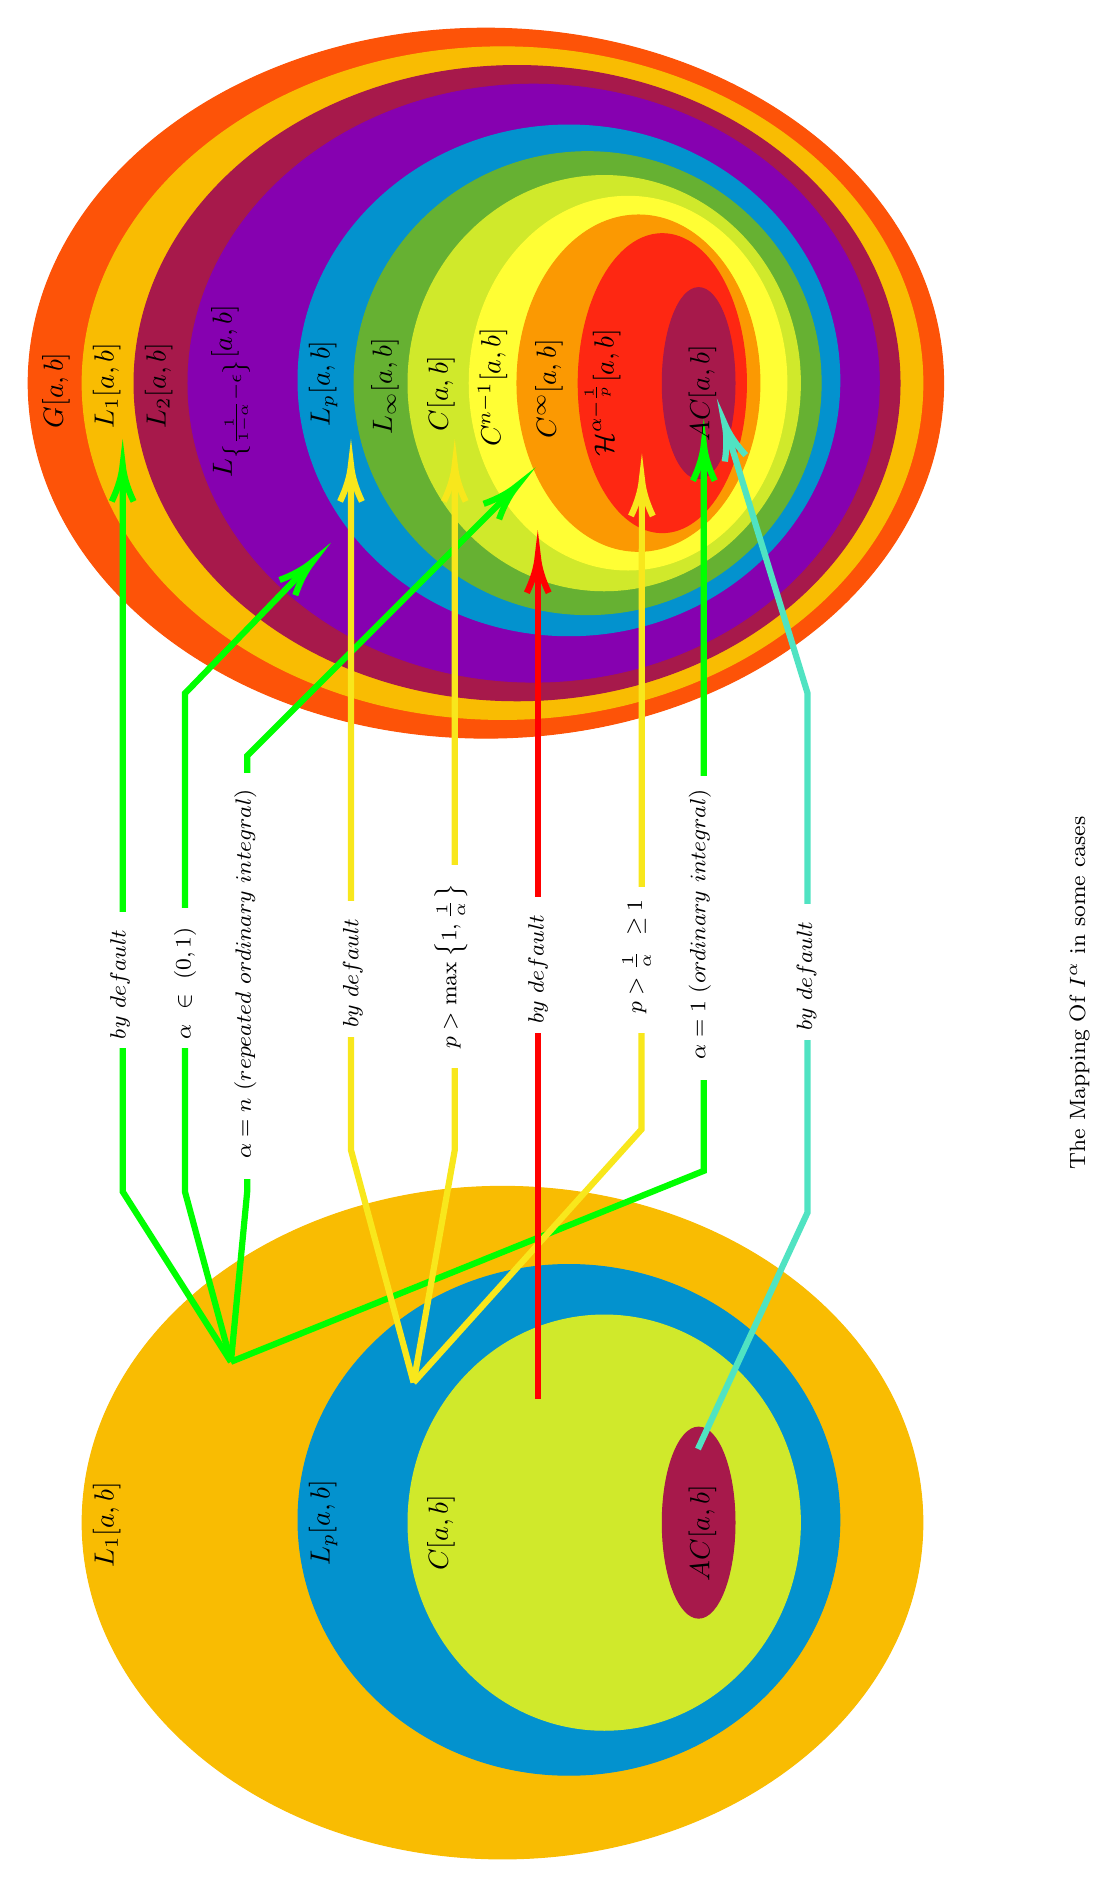
\begin{tikzpicture}[x=0.75pt,y=0.75pt,yscale=-1,xscale=1,scale=1]
%uncomment if require: \path (0,1171); %set diagram left start at 0, and has height of 1171

%Shape: Ellipse [id:dp36421966981860576] 
\draw  [color={rgb, 255:red, 253; green, 83; blue, 8 }  ,draw opacity=1 ][fill={rgb, 255:red, 253; green, 83; blue, 8 }  ,fill opacity=1 ] (320.5,376) .. controls (198.72,376) and (100,299.44) .. (100,205) .. controls (100,110.56) and (198.72,34) .. (320.5,34) .. controls (442.28,34) and (541,110.56) .. (541,205) .. controls (541,299.44) and (442.28,376) .. (320.5,376) -- cycle ;
%Shape: Ellipse [id:dp513596341046219] 
\draw  [color={rgb, 255:red, 249; green, 188; blue, 2 }  ,draw opacity=1 ][fill={rgb, 255:red, 249; green, 188; blue, 2 }  ,fill opacity=1 ] (328.5,367) .. controls (216.66,367) and (126,294.47) .. (126,205) .. controls (126,115.53) and (216.66,43) .. (328.5,43) .. controls (440.34,43) and (531,115.53) .. (531,205) .. controls (531,294.47) and (440.34,367) .. (328.5,367) -- cycle ;
%Shape: Ellipse [id:dp8342256600903095] 
\draw  [color={rgb, 255:red, 167; green, 25; blue, 75 }  ,draw opacity=1 ][fill={rgb, 255:red, 167; green, 25; blue, 75 }  ,fill opacity=1 ] (335.5,358) .. controls (233.6,358) and (151,289.5) .. (151,205) .. controls (151,120.5) and (233.6,52) .. (335.5,52) .. controls (437.4,52) and (520,120.5) .. (520,205) .. controls (520,289.5) and (437.4,358) .. (335.5,358) -- cycle ;
%Shape: Ellipse [id:dp7701966259035993] 
\draw  [color={rgb, 255:red, 134; green, 1; blue, 176 }  ,draw opacity=1 ][fill={rgb, 255:red, 134; green, 1; blue, 176 }  ,fill opacity=1 ] (343.5,349) .. controls (251.54,349) and (177,284.53) .. (177,205) .. controls (177,125.47) and (251.54,61) .. (343.5,61) .. controls (435.46,61) and (510,125.47) .. (510,205) .. controls (510,284.53) and (435.46,349) .. (343.5,349) -- cycle ;
%Shape: Ellipse [id:dp8718526137926743] 
\draw  [color={rgb, 255:red, 3; green, 146; blue, 206 }  ,draw opacity=1 ][fill={rgb, 255:red, 3; green, 146; blue, 206 }  ,fill opacity=1 ] (360.5,326.67) .. controls (288.43,326.67) and (230,271.6) .. (230,203.67) .. controls (230,135.74) and (288.43,80.67) .. (360.5,80.67) .. controls (432.57,80.67) and (491,135.74) .. (491,203.67) .. controls (491,271.6) and (432.57,326.67) .. (360.5,326.67) -- cycle ;
%Shape: Ellipse [id:dp07229888839358667] 
\draw  [color={rgb, 255:red, 102; green, 177; blue, 50 }  ,draw opacity=1 ][fill={rgb, 255:red, 102; green, 177; blue, 50 }  ,fill opacity=1 ] (369.5,316.5) .. controls (307.37,316.5) and (257,266.58) .. (257,205) .. controls (257,143.42) and (307.37,93.5) .. (369.5,93.5) .. controls (431.63,93.5) and (482,143.42) .. (482,205) .. controls (482,266.58) and (431.63,316.5) .. (369.5,316.5) -- cycle ;
%Shape: Ellipse [id:dp26102978707270297] 
\draw  [color={rgb, 255:red, 208; green, 233; blue, 43 }  ,draw opacity=1 ][fill={rgb, 255:red, 208; green, 233; blue, 43 }  ,fill opacity=1 ] (377.5,305) .. controls (325.31,305) and (283,260.23) .. (283,205) .. controls (283,149.77) and (325.31,105) .. (377.5,105) .. controls (429.69,105) and (472,149.77) .. (472,205) .. controls (472,260.23) and (429.69,305) .. (377.5,305) -- cycle ;
%Shape: Ellipse [id:dp3143329621107056] 
\draw  [color={rgb, 255:red, 255; green, 254; blue, 52 }  ,draw opacity=1 ][fill={rgb, 255:red, 255; green, 254; blue, 52 }  ,fill opacity=1 ] (389,295) .. controls (346.75,295) and (312.5,254.71) .. (312.5,205) .. controls (312.5,155.29) and (346.75,115) .. (389,115) .. controls (431.25,115) and (465.5,155.29) .. (465.5,205) .. controls (465.5,254.71) and (431.25,295) .. (389,295) -- cycle ;
%Shape: Ellipse [id:dp49451773436571855] 
\draw  [color={rgb, 255:red, 251; green, 153; blue, 2 }  ,draw opacity=1 ][fill={rgb, 255:red, 251; green, 153; blue, 2 }  ,fill opacity=1 ] (394,286) .. controls (361.69,286) and (335.5,249.74) .. (335.5,205) .. controls (335.5,160.26) and (361.69,124) .. (394,124) .. controls (426.31,124) and (452.5,160.26) .. (452.5,205) .. controls (452.5,249.74) and (426.31,286) .. (394,286) -- cycle ;
%Shape: Ellipse [id:dp7286874747001277] 
\draw  [color={rgb, 255:red, 254; green, 39; blue, 18 }  ,draw opacity=1 ][fill={rgb, 255:red, 254; green, 39; blue, 18 }  ,fill opacity=1 ] (405.5,277) .. controls (383.13,277) and (365,244.76) .. (365,205) .. controls (365,165.24) and (383.13,133) .. (405.5,133) .. controls (427.87,133) and (446,165.24) .. (446,205) .. controls (446,244.76) and (427.87,277) .. (405.5,277) -- cycle ;
%Shape: Ellipse [id:dp9160012222939253] 
\draw  [color={rgb, 255:red, 167; green, 25; blue, 75 }  ,draw opacity=1 ][fill={rgb, 255:red, 167; green, 25; blue, 75 }  ,fill opacity=1 ] (423,251) .. controls (413.34,251) and (405.5,230.41) .. (405.5,205) .. controls (405.5,179.59) and (413.34,159) .. (423,159) .. controls (432.66,159) and (440.5,179.59) .. (440.5,205) .. controls (440.5,230.41) and (432.66,251) .. (423,251) -- cycle ;

%Shape: Ellipse [id:dp7687741619822284] 
\draw  [color={rgb, 255:red, 249; green, 188; blue, 2 }  ,draw opacity=1 ][fill={rgb, 255:red, 249; green, 188; blue, 2 }  ,fill opacity=1 ] (328.5,916) .. controls (216.66,916) and (126,843.47) .. (126,754) .. controls (126,664.53) and (216.66,592) .. (328.5,592) .. controls (440.34,592) and (531,664.53) .. (531,754) .. controls (531,843.47) and (440.34,916) .. (328.5,916) -- cycle ;
%Shape: Ellipse [id:dp7863689832047069] 
\draw  [color={rgb, 255:red, 3; green, 146; blue, 206 }  ,draw opacity=1 ][fill={rgb, 255:red, 3; green, 146; blue, 206 }  ,fill opacity=1 ] (360.5,875.67) .. controls (288.43,875.67) and (230,820.6) .. (230,752.67) .. controls (230,684.74) and (288.43,629.67) .. (360.5,629.67) .. controls (432.57,629.67) and (491,684.74) .. (491,752.67) .. controls (491,820.6) and (432.57,875.67) .. (360.5,875.67) -- cycle ;
%Shape: Ellipse [id:dp36197594607695427] 
\draw  [color={rgb, 255:red, 208; green, 233; blue, 43 }  ,draw opacity=1 ][fill={rgb, 255:red, 208; green, 233; blue, 43 }  ,fill opacity=1 ] (377.5,854) .. controls (325.31,854) and (283,809.23) .. (283,754) .. controls (283,698.77) and (325.31,654) .. (377.5,654) .. controls (429.69,654) and (472,698.77) .. (472,754) .. controls (472,809.23) and (429.69,854) .. (377.5,854) -- cycle ;
%Shape: Ellipse [id:dp8626838071461165] 
\draw  [color={rgb, 255:red, 167; green, 25; blue, 75 }  ,draw opacity=1 ][fill={rgb, 255:red, 167; green, 25; blue, 75 }  ,fill opacity=1 ] (423,800) .. controls (413.34,800) and (405.5,779.41) .. (405.5,754) .. controls (405.5,728.59) and (413.34,708) .. (423,708) .. controls (432.66,708) and (440.5,728.59) .. (440.5,754) .. controls (440.5,779.41) and (432.66,800) .. (423,800) -- cycle ;


%Straight Lines [id:da29740484436841275] 
\draw [color={rgb, 255:red, 0; green, 255; blue, 0 }  ,draw opacity=1 ][line width=2.25]    (197.67,676.5) -- (145.5,594.5) -- (145.5,248.5) ;
\draw [shift={(145.5,244.5)}, rotate = 90] [color={rgb, 255:red, 0; green, 255; blue, 0 }  ,draw opacity=1 ][line width=2.25]    (17.49,-5.26) .. controls (11.12,-2.23) and (5.29,-0.48) .. (0,0) .. controls (5.29,0.48) and (11.12,2.23) .. (17.49,5.26)   ;
%Straight Lines [id:da747322555087151] 
\draw [color={rgb, 255:red, 0; green, 255; blue, 0 }  ,draw opacity=1 ][line width=2.25]    (197.67,676.5) -- (425.5,584.5) -- (425.5,238.5) ;
\draw [shift={(425.5,234.5)}, rotate = 90] [color={rgb, 255:red, 0; green, 255; blue, 0 }  ,draw opacity=1 ][line width=2.25]    (17.49,-5.26) .. controls (11.12,-2.23) and (5.29,-0.48) .. (0,0) .. controls (5.29,0.48) and (11.12,2.23) .. (17.49,5.26)   ;
%Straight Lines [id:da3355128348747227] 
\draw [color={rgb, 255:red, 0; green, 255; blue, 0 }  ,draw opacity=1 ][line width=2.25]    (197.67,676.5) -- (205.5,594.5) -- (205.5,384.5) -- (332.67,257.33) ;
\draw [shift={(335.5,254.5)}, rotate = 135] [color={rgb, 255:red, 0; green, 255; blue, 0 }  ,draw opacity=1 ][line width=2.25]    (17.49,-5.26) .. controls (11.12,-2.23) and (5.29,-0.48) .. (0,0) .. controls (5.29,0.48) and (11.12,2.23) .. (17.49,5.26)   ;
%Straight Lines [id:da5987549368234755] 
\draw [color={rgb, 255:red, 0; green, 255; blue, 0 }  ,draw opacity=1 ][line width=2.25]    (197.67,676.5) -- (175.5,594.5) -- (175.5,354.5) -- (234.27,293.82) ;
\draw [shift={(237.06,290.94)}, rotate = 134.08] [color={rgb, 255:red, 0; green, 255; blue, 0 }  ,draw opacity=1 ][line width=2.25]    (17.49,-5.26) .. controls (11.12,-2.23) and (5.29,-0.48) .. (0,0) .. controls (5.29,0.48) and (11.12,2.23) .. (17.49,5.26)   ;

%Straight Lines [id:da3971858139126001] 
\draw [color={rgb, 255:red, 248; green, 231; blue, 28 }  ,draw opacity=1 ][line width=2.25]    (285.67,686.5) -- (255.5,574.5) -- (255.5,248.5) ;
\draw [shift={(255.5,244.5)}, rotate = 90] [color={rgb, 255:red, 248; green, 231; blue, 28 }  ,draw opacity=1 ][line width=2.25]    (17.49,-5.26) .. controls (11.12,-2.23) and (5.29,-0.48) .. (0,0) .. controls (5.29,0.48) and (11.12,2.23) .. (17.49,5.26)   ;
%Straight Lines [id:da680452400138468] 
\draw [color={rgb, 255:red, 248; green, 231; blue, 28 }  ,draw opacity=1 ][line width=2.25]    (285.67,686.5) -- (305.5,574.5) -- (305.5,248.5) ;
\draw [shift={(305.5,244.5)}, rotate = 90] [color={rgb, 255:red, 248; green, 231; blue, 28 }  ,draw opacity=1 ][line width=2.25]    (17.49,-5.26) .. controls (11.12,-2.23) and (5.29,-0.48) .. (0,0) .. controls (5.29,0.48) and (11.12,2.23) .. (17.49,5.26)   ;
%Straight Lines [id:da03005347223035426] 
\draw [color={rgb, 255:red, 248; green, 231; blue, 28 }  ,draw opacity=1 ][line width=2.25]    (285.67,686.5) -- (395.5,564.5) -- (395.66,255.5) ;
\draw [shift={(395.67,251.5)}, rotate = 90.03] [color={rgb, 255:red, 248; green, 231; blue, 28 }  ,draw opacity=1 ][line width=2.25]    (17.49,-5.26) .. controls (11.12,-2.23) and (5.29,-0.48) .. (0,0) .. controls (5.29,0.48) and (11.12,2.23) .. (17.49,5.26)   ;

%Straight Lines [id:da15460774860319515] 
\draw [color={rgb, 255:red, 255; green, 0; blue, 0 }  ,draw opacity=1 ][line width=2.25]    (345.5,694.5) -- (345.5,292.5) ;
\draw [shift={(345.5,288.5)}, rotate = 90] [color={rgb, 255:red, 255; green, 0; blue, 0 }  ,draw opacity=1 ][line width=2.25]    (17.49,-5.26) .. controls (11.12,-2.23) and (5.29,-0.48) .. (0,0) .. controls (5.29,0.48) and (11.12,2.23) .. (17.49,5.26)   ;
%Straight Lines [id:da43732852110852893] 
\draw [color={rgb, 255:red, 80; green, 227; blue, 194 }  ,draw opacity=1 ][line width=2.25]    (422.67,718.5) -- (475.5,604.5) -- (475.5,354.5) -- (436.68,228.32) ;
\draw [shift={(435.5,224.5)}, rotate = 72.9] [color={rgb, 255:red, 80; green, 227; blue, 194 }  ,draw opacity=1 ][line width=2.25]    (17.49,-5.26) .. controls (11.12,-2.23) and (5.29,-0.48) .. (0,0) .. controls (5.29,0.48) and (11.12,2.23) .. (17.49,5.26)   ;


% Text Node
\draw (105.4,228) node [anchor=north west][inner sep=0.75pt]  [rotate=-270]  {$G[ a,b]$};
% Text Node
\draw (129.9,228) node [anchor=north west][inner sep=0.75pt]  [rotate=-270]  {$L_{1}[ a,b]$};
% Text Node
\draw (154.9,228) node [anchor=north west][inner sep=0.75pt]  [rotate=-270]  {$L_{2}[ a,b]$};
% Text Node
\draw (263.9,231) node [anchor=north west][inner sep=0.75pt]  [rotate=-270]  {$L_{\infty }[ a,b]$};
% Text Node
\draw (233.9,227) node [anchor=north west][inner sep=0.75pt]  [rotate=-270]  {$L_{p}[ a,b]$};
% Text Node
\draw (290.9,229.5) node [anchor=north west][inner sep=0.75pt]  [rotate=-270]  {$C[ a,b]$};
% Text Node
\draw (366.9,241.5) node [anchor=north west][inner sep=0.75pt]  [rotate=-270]  {$\mathcal{H}^{\alpha -\frac{1}{p}}[ a,b]$};
% Text Node
\draw (416.9,234.5) node [anchor=north west][inner sep=0.75pt]  [rotate=-270]  {$AC[ a,b]$};
% Text Node
\draw (342.9,233) node [anchor=north west][inner sep=0.75pt]  [rotate=-270]  {$C^{\infty }[ a,b]$};
% Text Node
\draw (315.4,237) node [anchor=north west][inner sep=0.75pt]  [rotate=-270]  {$C^{n-1}[ a,b]$};
% Text Node
\draw (186.9,251.5) node [anchor=north west][inner sep=0.75pt]  [rotate=-270]  {$L_{\left\{\frac{1}{1-\alpha } -\epsilon \right\}}[ a,b]$};
% Text Node
\draw (129.9,777) node [anchor=north west][inner sep=0.75pt]  [rotate=-270]  {$L_{1}[ a,b]$};
% Text Node
\draw (233.9,776) node [anchor=north west][inner sep=0.75pt]  [rotate=-270]  {$L_{p}[ a,b]$};
% Text Node
\draw (290.9,778.5) node [anchor=north west][inner sep=0.75pt]  [rotate=-270]  {$C[ a,b]$};
% Text Node
\draw (416.9,783.5) node [anchor=north west][inner sep=0.75pt]  [rotate=-270]  {$AC[ a,b]$};
% Text Node
\draw  [color={rgb, 255:red, 255; green, 255; blue, 255 }  ,draw opacity=1 ][fill={rgb, 255:red, 255; green, 255; blue, 255 }  ,fill opacity=1 ]  (279.94,437.61) -- (327.94,437.61) -- (327.94,534.61) -- (279.94,534.61) -- cycle  ;
\draw (294.34,527) node [anchor=north west][inner sep=0.75pt]  [font=\footnotesize,rotate=-270]  {$p >\max\left\{1,\frac{1}{\alpha }\right\}$};
% Text Node
\draw  [color={rgb, 255:red, 255; green, 255; blue, 255 }  ,draw opacity=1 ][fill={rgb, 255:red, 255; green, 255; blue, 255 }  ,fill opacity=1 ]  (335.28,452.94) -- (355.28,452.94) -- (355.28,517.94) -- (335.28,517.94) -- cycle  ;
\draw (339.68,514.94) node [anchor=north west][inner sep=0.75pt]  [font=\footnotesize,rotate=-270]  {$by\ default$};
% Text Node
\draw  [color={rgb, 255:red, 255; green, 255; blue, 255 }  ,draw opacity=1 ][fill={rgb, 255:red, 255; green, 255; blue, 255 }  ,fill opacity=1 ]  (464.61,456.28) -- (484.61,456.28) -- (484.61,521.28) -- (464.61,521.28) -- cycle  ;
\draw (469.01,518.28) node [anchor=north west][inner sep=0.75pt]  [font=\footnotesize,rotate=-270]  {$by\ default$};
% Text Node
\draw  [color={rgb, 255:red, 255; green, 255; blue, 255 }  ,draw opacity=1 ][fill={rgb, 255:red, 255; green, 255; blue, 255 }  ,fill opacity=1 ]  (245.94,454.94) -- (265.94,454.94) -- (265.94,519.94) -- (245.94,519.94) -- cycle  ;
\draw (250.34,516.94) node [anchor=north west][inner sep=0.75pt]  [font=\footnotesize,rotate=-270]  {$by\ default$};
% Text Node
\draw  [color={rgb, 255:red, 255; green, 255; blue, 255 }  ,draw opacity=1 ][fill={rgb, 255:red, 255; green, 255; blue, 255 }  ,fill opacity=1 ]  (133.85,460.28) -- (153.85,460.28) -- (153.85,525.28) -- (133.85,525.28) -- cycle  ;
\draw (138.25,522.28) node [anchor=north west][inner sep=0.75pt]  [font=\footnotesize,rotate=-270]  {$by\ default$};
% Text Node
\draw  [color={rgb, 255:red, 255; green, 255; blue, 255 }  ,draw opacity=1 ][fill={rgb, 255:red, 255; green, 255; blue, 255 }  ,fill opacity=1 ]  (164.52,458.28) -- (184.52,458.28) -- (184.52,525.28) -- (164.52,525.28) -- cycle  ;
\draw (168.92,522.28) node [anchor=north west][inner sep=0.75pt]  [font=\footnotesize,rotate=-270]  {$\alpha \ \in \ ( 0,1)$};
% Text Node
\draw  [color={rgb, 255:red, 255; green, 255; blue, 255 }  ,draw opacity=1 ][fill={rgb, 255:red, 255; green, 255; blue, 255 }  ,fill opacity=1 ]  (374.17,447.94) -- (411.17,447.94) -- (411.17,517.94) -- (374.17,517.94) -- cycle  ;
\draw (385,510) node [anchor=north west][inner sep=0.75pt]  [font=\footnotesize,rotate=-270]  {$p >\frac{1}{\alpha } \ \geq 1$};
% Text Node
\draw  [color={rgb, 255:red, 255; green, 255; blue, 255 }  ,draw opacity=1 ][fill={rgb, 255:red, 255; green, 255; blue, 255 }  ,fill opacity=1 ]  (415.28,394.61) -- (435.28,394.61) -- (435.28,540.61) -- (415.28,540.61) -- cycle  ;
\draw (417,532) node [anchor=north west][inner sep=0.75pt]  [font=\footnotesize,rotate=-270]  {$\alpha =1\ ( ordinary\ integral)$};
% Text Node
\draw  [color={rgb, 255:red, 255; green, 255; blue, 255 }  ,draw opacity=1 ][fill={rgb, 255:red, 255; green, 255; blue, 255 }  ,fill opacity=1 ]  (196.08,392.94) -- (216.08,392.94) -- (216.08,587.94) -- (196.08,587.94) -- cycle  ;
\draw (198,580) node [anchor=north west][inner sep=0.75pt]  [font=\footnotesize,rotate=-270]  {$\alpha =n\ ( repeated\ ordinary\ integral)$};
\draw (600.48,584.94) node [anchor=north west][inner sep=0.75pt]  [font=\footnotesize,rotate=-270]  {The Mapping Of $I^{\alpha}$ in some cases};

\end{tikzpicture}


\newpage


